\section{Group Theory} 
One of the most fundamental algebraic structures is called a group. A group is defined by an underlying set and one binary operation on elements of this set. An example of a group would be the integer numbers with addition as the operation. One typically denotes a group as a pair (in the sense of 2-tuple) consisting of the set and the operation, so the group of integers with addition is denoted by $(\mathbb{Z},+)$. Let's abstract from this concrete example and consider an arbitrary set $G$ on which an arbitrary binary operation, denoted by $\circ$, is defined and consider the pair $(G,\circ)$. For such a pair to qualify as a group, the operation $\circ$ has to satisfy the following rules which we henceforth will call the group axioms:

\medskip
\begin{tabular}{l l}
Closure: 
& $\forall a,b \in G: \; a \circ b \in G$  \\	
Associativity: 
& $\forall a,b,c \in G: \;  (a \circ b) \circ c = a \circ (b \circ c)$   \\
Existence of neutral element: 
& $\exists e \in G: \; (\forall a \in G: e \circ a = a)$ \\
Existence of inverse elements: 
& $\forall a \in G: \; (\exists a^{-1} \in G: a^{-1} \circ a = e )$ \\
\end{tabular}
\medskip

Let's translate that foreign mathspeak to plain English: \emph{Closure} means that when we combine any two elements $a,b$ from our set with the operation $\circ$, the result will be another element from the set. We also say that the set is \emph{closed} under the given operation. Sometimes, this first rule is not even explicitly stated as such but just somehow implicitly assumed by saying that the binary operation is an operation \emph{on} the set where the "on" here means that both inputs and the output have to be \emph{in} the set. If not explicitly stated, the closure property is hidden in the definition of what is considered to be viable as "binary operation", so to speak. But if one allows a more general notion of what a binary operation is, allowing inputs and outputs to come from different sets: $op: A \times B \rightarrow C$, it makes sense to explicitly require this closure property. \emph{Associativity} requires that when we combine 3 elements $a,b,c$ via our operation by firstly combining $a$ and $b$ and then secondly combining the result of that with $c$ yields the same final result as combining $a$ with the result of the combination of $b$ and $c$. This is an abstraction of the idea that $(2+3)+4 = 2+(3+4)$ because $5+4 = 2+7$. The second rule says that there must exist some special element $e$ within the set which, when combined with any element $a$ from the set, just gives back $a$ itself. This special element $e$ is called the \emph{neutral element} because it changes nothing when it's being combined with any element from the set. It's an abstraction of the idea that $0+x = x$ for any $x$ whatsoever. The number zero is the neutral element of addition in the integers. At the outset, it may seem that we should actually be more precise and call it the left-neutral element because we require it to behave neutrally only from the left. However, group theory gives us the theorem that any left-neutral element is automatically always also right-neutral, so it's justified to just call it the neutral element without any left or right qualifier. Group theory also gives us the theorem that such a neutral element is always unique so it's indeed justified to call it \emph{the} neutral element instead of \emph{a} neutral element. By the way, it is common to refer by the term "group" also to the underlying set rather than the pair if it's clear from the context about which operation we talk. The last rule requires that for any element $a$ from the group there must exist some element $a^{-1}$, also from the group, such that when we form the combination $ a^{-1} \circ a$ via our group operation, then the neutral element will come out as result. This element $a^{-1}$ is called the \emph{inverse element} to $a$. So, the rule says that such inverse elements must exist for all group elements. In the integers with addition, the inverse element to $3$ is $-3$ because $-3 + 3 = 0$ where zero is the neutral element as we have established before. Again, we need to require only the existence of left-inverses and group theory assures us by way of a theorem that any left-inverse element is proven to always automatically also be right-inverse and is unique so we are justified to call it "the inverse element" and not just "a left-inverse element". We may begin to see the value of group theory. If we want to verify that right-inverses exist in some brand new mathematical structure that we came up with, we actually just need to check these three simple conditions and if they hold true, we are good and can in fact assert a lot more properties of our structure without needing to verify them all separately. 

\paragraph{Notation and Terminology}
So far, we have used the symbol $\circ$ in infix notation like in $c = a \circ b$ to denote the combination of elements $a,b$ by our group operation. This was done to indicate that we don't not necessarily mean a concrete well known operation such as addition or multiplication. Depending on the context, the group operation may indeed be addition. Or it may be multiplication. Or something else entirely. It may also mean the composition of certain \emph{actions} in the sense of performing one action after another. We may be used to the circle being used for function composition and indeed, if we consider only invertible (i.e. strictly monotonic) functions, they do indeed form a group under function composition (where "under" here means: "with the group operation being"). This usage of the circle is not universal. You will also often encounter the dot being used: $c = a \cdot b$ and sometimes the operation symbol is scrapped entirely: $c = a b$ like we often do with multiplication when dealing with numbers, matrices, functions and so on. From now on, we will also adopt these notations. We will also denote the combination of an element $a$ with itself as $a^2$, i.e. $a^2 = a a = a \cdot a$. In general we will denote by $a^n$ the idea to combine $a$ with itself $n-1$ times. That is, we have $n$ "factors" all of them being $a$ and we have $n-1$ "dots" in between them: $a^4 = a \cdot a \cdot a \cdot a$. The group operation is sometimes just called "multiplication" even though it is understood that a generalized, more abstract operation is meant. In the definition of a group, we did not require the operation to be commutative. However, if the operation does happen to be also commutative, i.e. if $a b = b a$ for all $a,b \in G$, then we call the group a \emph{commutative} group or some people also call it an \emph{Abelian} group. I prefer use descriptive names whenever possible - no offense to Niels Henrik Abel (hopefully). In such a commutative group, it makes no difference whether we pre- or post-multiply by an element. This holds of course also for inverses, so $c = b^{-1} a$ is equivalent to $c = a b^{-1}$ for any $a,b \in G$. That's why, for commutative groups, you'll sometimes find the division notation $c = \frac{a}{b}$ because the inherent ambiguity in this notation about whether pre- or post-multiplication of $a$ by $b^{-1}$ is meant, makes no difference because both ways yield the same result anyway. We won't use that notation here, though because we won't assume our groups to be commutative in general. If we are dealing with such a commutative group, we will have even more theorems at our disposal. When we are dealing with a group that is not generally commutative, it may still happen that for some specific choice of $a,b$ the equation $a b = b a$ holds. In such a case, we say that "$a$ and $b$ commute". The number of elements in a group's underlying set is called the \emph{order} of the group.
% Maybe use the dot right from the start...maybe not
% Commutators make sense only in rings later, I think because we need the two operations to even define it - so don't mention it here - mention it later in the Ring Theory chapter






%===================================================================================================
\subsection{Some Elementary Theorems}
Let's axiomatically assume that our rules stated above are true for some given pair of a set and an operation that is of interest to us. Let's say, we have painstakingly verified them by hand and have convinced ourselves that our pair does indeed form a group. What else can we deduce from the group axioms alone without knowing anything more about our pair other than it being a group? What other properties can we assert about our pair without actually verifying them by hand? Without proof, I'll hand you down the following useful facts for any group, some of which were already mentioned: 
\begin{enumerate}
\item Neutral and inverse elements are unique. 

\item Left neutral elements are also right-neutral and left-inverses are also right-inverse. If $a^{-1} a = e$ then $a a^{-1} = e$. Note that this does \emph{not} imply that pre- or post-multiplying any \emph{other} element by an inverse makes no difference! It \emph{does} make a difference, i.e. $a^{-1} b \neq b a^{-1}$ in general unless the group is commutative. It only says that $a$ and $a^{-1}$ commute but any other $b$ may not commute with $a^{-1}$.

\item We have general rules for exponents: $a^m a^n = a^{m+n}$ and $(a^{m})^{n} = (a^{n})^{m} = a^{n m}$. As a special case of this, we have the rule that inverting twice gives back the original: $(a^{-1})^{-1} = a$ because $(-1) \cdot (-1) = 1$.

\item In a power of a sandwich of the form $a^{-1} b a$, we can drag the exponent in to apply only to $b$: $(a^{-1} b a)^{-1} = a^{-1} b^n a$. This useful in the context of matrix exponentiation via diagonalization.

\item If $a$ and $b$ commute, i.e. if we have $a b = ba$ then we also have: $(a b)^n = a^n b^n = b^n a^n$ and $a b^n = b^n a$. In commutative groups, all $a,b$ commute so there, these laws hold for any $a,b$.

\item An inverse of a product is the product of the inverses in reverse order: $(a b c)^{-1} = c^{-1} b^{-1} a^{-1}$. I've written it down for three factors but it holds for any number of factors. In a commutative group, the order doesn't even matter so we can freely rearrange the factors however we like [VERIFY!]. 

\item The cancellation law says that if $a b = a c$ then $b = c$. We can cancel the $a$ from both sides. This works also for right-multiplication: if $b a = c a$ then $b = c$. 

\item If we have an equation like $a x = b$ with known $a, b$ and unknown $x$, we can solve for $x$ by pre-multiplying both sides with $a^{-1}$ to get $x = a^{-1}b$. Likewise, if the equation is $x a = b$, we can solve for $x$ by post-multiplying by $a^{-1}$ to get $x = b a^{-1}$. 
\end{enumerate}

\medskip
I hope you will agree that these are quite a lot of potentially useful facts. Especially the ability to solve equations for unknowns  may be a big boon in many situations. Some of these facts may not be immediately obvious. But they have been proven from the group axioms alone, so they \emph{will} hold for \emph{your} group, if it indeed is a group, i.e. if you were able to verify the 4 simple requirements. There are many more facts to come that your group will also automatically satisfy just by virtue of being a group. That is why we are doing all of this - so you don't have to. Abstract algebra is about avoiding duplication of work. Sorry, if I sometimes fall into the habit of sounding like one of those annoying motivational speakers. But being the lazy person that I am, I really appreciate the avoidance of duplication of work. ;-) It's all about automation and efficiency. About working smart instead of working hard. About doing things once and for all instead of again and again. The art and craft of this is to abstract and distill out those features that actually matter and are applicable to as many concrete problems as possible. It turns out that especially associativity is such an important property for an operation to have because it allows us to turn a binary operation in a well defined way into an operation that can operate on any number of inputs by a process that is known as "fold" or "reduce" in the realm of functional programming. You start with a list of operands, then combine the first two elements via the operation, then combine the result of that with the third element and so on. Associativity guarantees that in such a folding, the order of the elements within the list doesn't matter such that the operation is well defined on any number of inputs without having to consider the order of the inputs.
%by "folding" a repeatedly applied binary operation as in "reduce" in functional programming

%https://www.cs.utoronto.ca/~szhao/group_theory_thms_defs.pdf
%Nice list of elementary facts

\medskip

%(8) The division axiom states that given any pair of elements $a,b$, there exist unique group elements $x,y$ such that $a x = b$ and $y a = b$, namely $x = a^{-1} b$ and $y = b a^{-1}$ [VERIFY!]. That means, we can solve equations for unknown variables. (see Riley/Hobson et al)

% partially obsolete?:
%\medskip
%\begin{tabular}{l l}
%Neutral elements are unique \\
%Inverse elements are unique \\	
%Left-neutral elements are also right-neutral \\
%Left-inverse elements are also right-inverse \\
%Inverses of inverses give back the original: & $(a^{-1})^{-1} = a$ \\
%Inverse of the square is square of inverse: & $(a^{2})^{-1} = (a^{-1})^{2} $ \\
%More generally - rule for exponents: & $(a^{m})^{n} = (a^{n})^{m} = a^{n m} $ \\
%\end{tabular}
%\medskip
% -uniqueness of inverses and neutral element
% -power rules
% In this context, it is natural to define $a^0 = e$.
% Q: 
% -could there be elements that are partially neutral, i.e. leave only some elements
%  unchanged but not all?

% https://math.stackexchange.com/questions/2930287/exponent-rules-under-a-group-g
% https://math.stackexchange.com/questions/2199421/do-the-laws-of-exponents-apply-to-a-group-as-for-real-numbers
% https://mathstats.uncg.edu/sites/pauli/112/HTML/secgroupexp.html

%===================================================================================================
\subsection{Groups and Symmetries}
One will often hear the statement that groups are an abstraction of \emph{symmetry}. A symmetry is, by definition, some transformation of an object that leaves some property of interest unchanged. Consider a square. We may rotate it by any integer multiple of 90 degrees around its center (including zero and negatives) and we may also reflect it horizontally, vertically or diagonally - all without changing its shape. In this setting, the rotations and reflections would be thought of as being the members of our group and the group operation would be to compose these transformations. It may be verified that our four rules do indeed hold true for this set of transformations, so it is indeed a group. When we say that these transformations act on the square, it may be not entirely clear, how we would "implement" such an action. We could imagine the square to live in 2D Euclidean space centered at the origin. Then, a square could be represented by 4 coordinate vectors for its 4 vertices, e.g. $(1,1),(-1,1),(-1,-1),(1,-1)$. In this setup, we would represent the transformations as matrices that can act on these vectors. This is the sort of stuff that we do in analytic geometry. Instead of thinking about the transformations as acting on vertices, we could also imagine it to act on the 2D space as whole. We should also specify what we mean by saying "the shape stays the same". In geometry, shapes of polygons are captured by the mutual distances between all the vertices. If an object is represented by a set of vertices and we apply a transformation to each vertex and after that transformation, the distances between all the vertices are the same as before, then the shape and size of the object has not changed. That's how we can verify that our transformation is indeed a symmetry for the given polygon. To recap: in this case, the group members are certain geometric transformations (reflections and rotations), the object on which the group acts is a square and the invariant property is the shape (captured in the mutual distances).
% It should perhaps be explained that by applying the transformation to the vertices, we apply it only to the coordinates by we somehow keeop our indexing of the vertices fixed. I mean, *any* Euclidean transformation would be a symmetry to *any* polygon if we do not somehow fix the vertices. I mean it in the sense that, if initially we have A=(1,1)=top-right, B=(-1,1)=top-left, C=(-1,-1)=bottom-left, D=(1,-1)=bottom-right, then after the horizontal flip we have A in the top-left, etc. if we also "reflect the labels" along with the cooridinates. But, I think, to verify that the shape is the same, we need to consider the invariance of the distances between the new coordinateas but without reflecting the labels...don't know how to express this in a way that makes sense - think about it! ...I think, we must permute only the cooridnates but not the labels/indices. ..or well...no - the idea of "reflecting the labels" makes not sense anyway.

%\subsubsection{The Group Action} I have informally used phrases like "the group element acts on" some object. This notion of "acting on" can be formalized as follows ...TBC... [TODO: maybe make it a section, include orbit-stabilizer theorem]

% https://en.wikipedia.org/wiki/Group_action
% https://mathworld.wolfram.com/GroupAction.html
%
% https://www.youtube.com/watch?v=EsBn7G2yhB8&list=PLDcSwjT2BF_VuNbn8HiHZKKy59SgnIAeO
% 2:58: Group Action definition
% ...says that the normal order is to put it somewhere after Lagrange's Theorem
%
% Maybe make it a section - either before Generators or before Morphisms
%
% https://en.wikipedia.org/wiki/Group_action#Orbits_and_stabilizers
%
% Orbit-Stabilizer Theorem:
%   orb(x)   = \{ g(x) : g \in G  \}        set of objects that x can get mapped to
%   stab(x)  = \{ g \in G : g(x) = x \}     set of trafos that leave x fixed
% Theorem: |G| = |orb(x)| \cdot |stab(x)|  \forall x \in X
% Other facts of interets:
% -stab(x) is a subgroup of G also denoted as G_x
% -something about equivalence classes?
%
% -We use function application notation g(x) to denote the action of g on x. We interpret g as a
%  function that is applied to x.
% -x is an element of X where X is the set of objects on which G acts.

\medskip
I find the statement "groups are an abstraction of symmetry" a bit confusing because it seems to be unnecessarily restrictive and complicated. The restriction is to view the group elements as transformations. We didn't say anything about such an interpretation in our axioms. Previously, they were just some arbitrary set elements. The complication is that we needed to introduce an auxiliary set, namely the set of \emph{objects} that the transformations \emph{act on}. We didn't say anything about such "objects" in our axioms. So, our definition of a group as a set together with an operation that satisfies certain rules, is both simpler and more general than the view as "abstraction of symmetry". The downside of being more general is that it is also more abstract. Anyway, let's see if we can interpret the group $(\mathbb{Z},+)$ within that mental image of symmetries. We want to interpret elements of $\mathbb{Z}$ as transformations that act on some object or set of objects. The elements of $\mathbb{Z}$ are integer numbers. They could act on other numbers by shifting (aka translating) them. We could also imagine them to act on the whole number line all at once. The number 5 shifts the number line to the right by five units, the number $-2$ shifts it to the left by two units. When we combine $5$ and $-2$ by our group operation (which is addition in this case), we obtain $3$ which represents a shift of the number line by $3$ units to the right. For a transformation to be a symmetry, we also need to specify the property that remains invariant under the transformation. In this case, this invariant property is the distance between pairs of numbers. When we imagine the shift transformation not to act on the number line as a whole but on single numbers, then the set of group elements is actually the same as the set of objects on which the group elements act. It may be confusing here that the set of objects and the set of actions is actually the same set but interpreted in two different ways namely as positions (objects) and as translations (actions). The objects and the actions have different roles and do not need to come from the same set in general. The rotations and reflections (actions) on the one hand and the  vertices (objects) on the other hand from the square example are certainly different things. A (rotation or reflection) matrix has a different data type than a vertex (i.e. a point or vector). It may also be confusing that the group operation, namely addition of numbers, seems to be the same operation as the group action - the shifting of the number line is also achieved by addition. That is also a coincidence in the case of the specific group $(\mathbb{Z},+)$. For the rotations and reflections of the square, the group operation would be composition (implemented as matrix multiplication) whereas the group action would be application (implemented as matrix-times-vector product). In some groups, we may identify the group members themselves with members of the set on which they act - objects and actions are kinda the same thing. 

% ...but I think there is always some sort of homomorphism by which we can do such an identification of group members with members of the set that is acted on? Figure out! maybe mention it. Or maybe not - it may just add confusion to talk about things like homomorphisms at this stage.

%In other groups, we can't do this.

% or can we - see this video at 38:01
% https://www.youtube.com/watch?v=UhE0t3SP6E8
% We can identify group elements with bijective maps from the group to itself. What about the rotations. normally, they act on R^2. But we may also let them act on the rotations themselvse. Then we get a permutation group

% Is it true that when we can identify objects with actions, we can also always identify the group operation with the group action? Stated another way: can we find a group where we can identify objects with actions but can't identify the group operation with the group action?

% https://www.youtube.com/watch?v=mvmuCPvRoWQ





%===================================================================================================
\subsection{Multiplication Tables}
Let's assume that we have a finite set $A$ with $N$ elements and let's assume that we have labeled all set elements by a unique index between $1$ and $N$, so our set is $A = \{ a_1, a_2, a_3, \ldots, a_N \}$. To define a binary operation on such a set, we may write down a table in which the headers of the rows and columns are the set elements and the cells tell us, what output the operation will produce, when we combine the elements that appear in the headers of our rows and columns. That means, when we view the table as a matrix $T$, the element $t_{ij}$ of the matrix will be given by the product $a_i a_j$. I call it a "matrix" here because that's the data structure one might naturally want to use for this in an (naive) implementation - but we do not intend to do any linear algebra with it. For our purposes here, it's just a 2D table of elements which we want to read out and I may use the terms "matrix" and "table" interchangably. For $N=5$, such a table would look like this:
\[
\setlength{\extrarowheight}{5pt}% local setting
\begin{array}{l|*{5}{c}}
	    & a_1   & a_2  & a_3 & a_4  & a_5 \\
	\hline
	a_1 & a_1 a_1 & a_1 a_2 & a_1 a_3 & a_1 a_4  & a_1 a_5 \\
	a_2 & a_2 a_1 & a_2 a_2 & a_2 a_3 & a_2 a_4  & a_2 a_5 \\
	a_3 & a_3 a_1 & a_3 a_2 & a_3 a_3 & a_3 a_4  & a_3 a_5 \\
	a_4 & a_4 a_1 & a_4 a_2 & a_4 a_3 & a_4 a_4  & a_4 a_5 \\
	a_5 & a_5 a_1 & a_5 a_2 & a_5 a_3 & a_5 a_4  & a_5 a_5 \\
\end{array} 
\]
This table is supposed to represent the results of our group operation. From the row header, we take the left factor $a_i$, from the column header, we take the right factor $a_j$ and into the cell $t_{ij}$, we write the product $a_i a_j$. Again, I say "factor" and "product" but actually mean it in a more general and abstract sense as "operand" and "result". Such a table of all possible products of group elements is called a multiplication table, also known as Cayley table. By using such tables, we have a completely general way to specify any binary operation on a finite set of elements. We just need to define an indexing scheme for our set elements and then write the values of all possible products into the cells of the table. It is customary to write the neutral element into the header of the first row and first column.

\medskip
Now, for the table to specify an operation that does satisfy our group requirements, it must satisfy some constraints. Firstly, it must be a so called Latin square which is a matrix in which each row and each column contains every element from the set exactly once. That this is necessary can be seen as follows: suppose you know a product $p = a_i a_j$ and you also know one of the factors, say $a_i$. Then, it should be possible to find the other factor $a_j = a_i^{-1} p$ by scanning the row of $a_i$ until you find $p$ and then read off the column header where you found it. That must be $a_j$. But for that to work for any $p \in G$, you can't have duplicate elements on the rows because then you wouldn't know, which column header you should read off - and hence, the product is not uniquely invertible. This is not allowed in a group. Another constraint is that there must be some row and column that just lists the elements in the same order as they appear in the header - that's the row/column of the neutral element. They must cross on the diagonal, i.e. row and column index must be the same. These criteria are rather easy to check. If they fail, the table is not a valid multiplication table. But if they hold, the table could still be invalid. These criteria are necessary but not sufficient. We also need to verify the associativity and that's the hard part. Of course, it can naively be verified algorithmically in $\mathcal{O}(N^3)$ by verifying for every possible triple $a_i, a_j, a_k$ that $(a_i a_j) a_k = a_i (a_j a_k)$. There are algorithms that can do better than that in certain cases (search for "Light's associativity test") but as of now, this seems indeed to be an $\mathcal{O}(N^3)$ problem in terms of worst case complexity.

\medskip
But be that as it may. Multiplication tables are an important tool in the analysis of finite groups because these tables completely specify (and hopefully reveal) the structure of a given group at hand. For example, we may easily find out whether or not a group is \emph{commutative}. This is the case, if and only if the multiplication table is \emph{symmetric} across the main diagonal. But as we will see when we come to the topic of subgroups, finite groups can have more structure than that. But after all that abstract stuff, let's first have a look at...

% Not every Latin square is a Cayley table:
% https://proofwiki.org/wiki/Latin_Square_is_not_necessarily_Cayley_Table_of_Group

% https://math.stackexchange.com/questions/1297564/verifying-if-a-multiplication-table-is-from-a-group

% https://math.stackexchange.com/questions/168663/is-there-an-easy-way-to-see-associativity-or-non-associativity-from-an-operation

% https://en.wikipedia.org/wiki/Light's_associativity_test

% Q: Does it actually make any sense to do linear algebra with Caley tables? If we have two Caley tables of two different groups (of the same size) - what is their product? Will it also be a Caley table of a group? ...maybe try it with some examples. I guess that would mean that Latin squares would need to form a subgroup of the group of all matrices under matrix multipication. Do they? ...naaahhh...that doesn't make any sense!
% https://en.wikipedia.org/wiki/Latin_square
%===================================================================================================
\subsection{Some Examples}
Now that we have defined what a group is in an abstract sense and have a tool in hand to specify a group, let's look at some concrete examples of very different groups to get an appreciation for how surprisingly universally applicable these concepts are.

\subsubsection{Numbers}
We have already mentioned that the integer numbers form a group under addition. So do the rational numbers, real numbers and complex numbers. So, in math notation that means:  $(\mathbb{Z}, +), (\mathbb{Q}, +), (\mathbb{R}, +), (\mathbb{C}, +)$ all form groups. These latter three number systems also form groups under multiplication if we remove the number zero. If we denote by a superscript asterisk the set with the zero removed, for example $\mathbb{Q}^{\ast} = \mathbb{Q} \setminus \{0\}$, then we can state with math notation: The pairs $(\mathbb{Q}^{\ast}, \cdot), (\mathbb{R}^{\ast}, \cdot), (\mathbb{C}^{\ast}, \cdot)$ also form groups. If we want to interpret these multiplicative group as symmetries, then the invariant property would be the ratio of pairs of numbers. A bit less familiar, but very important in number theory and some areas of computer science are the modular integers. I don't want to digress too much into explaining what they are here at this point, but if you know what they are, then let me tell you that they also do form groups under modular addition. If the modulus is prime, they also form groups under modular multiplication when the zero is removed. They actually even form fields in this case - a more complex algebraic structure that we will encounter later. %There are many more number systems that have the structure of a group and often even more complex structures. 

\subsubsection{Matrices}
Consider the set of all regular (i.e. invertible) $n \times n$ matrices for some $n$. This set forms a group under matrix multiplication. This group is clearly not commutative because we know that matrix multiplication isn't. You may find many different subsets of this group of \emph{all} invertible matrices which are closed under matrix multiplication and inversion and which contain the identity matrix. These subsets may be finite or infinite. Let's take $n=2$. A simple example for a finite subset of that kind is given by the set of matrices that rotate by multiples of 90 degrees:
\begin{equation}
r^0 = \begin{pmatrix}  1 &  0 \\  0  &  1  \end{pmatrix}, \;
r^1 = \begin{pmatrix}  0 & -1 \\  1  &  0  \end{pmatrix}, \;
r^2 = \begin{pmatrix} -1 &  0 \\  0  & -1  \end{pmatrix}, \;
r^3 = \begin{pmatrix}  0 &  1 \\ -1  &  0  \end{pmatrix}
\end{equation}	
I have suggestively written the index as superscript like an exponent because they are indeed all powers of $r^1$. We see a little bit of foreshadowing to generators here. The element $r^1$ generates the whole group via its powers. Note also that $r^2$ is the negative identity matrix. It's a sort of $-1$ within the realm of matrices. Note furthermore that $r^1$ squares to $r^2$. That means $r^1$ behaves like an imaginary unit. That's no coincidence. If we consider the vector space spanned by $r^0$ and $r^1$, we get something that is completely isomorphic to the complex numbers [VERIFY!]. But that's just an aside. The important takeaway for the context of group theory is that there exist interesting subsets of the big set of all $n \times n$ matrix that exhibit the structure of a group. An example of an infinite set of that kind would be the set of all 2D rotation matrices where the angle can be any real number. That set happens to be isomorphic to all complex numbers with unit magnitude, i.e. complex numbers of the form $e^{\i \theta}$ for some real number $\theta$ that is interpreted as angle. Rotations in higher dimensions also form groups. Also of interest are matrices over the complex numbers. We'll hear more about all of that in the section about Lie groups.

% Maybe introduce a bit of jargon like SO(2), SU(2), ...but maybe do that in a later section about Lie groups

% Maybe mention that the group consists topologically of two disconnected parts because when going from positive to negative determinants we must cross the matrices with zero determinant which do not belong to the set. It's like with the multiplicative group of real numbers. The number zero is removed and therefore splits the set of numbers into disconnected segments (maybe mention that in the paragraph about numbers already). I think, the boundary between the two segments is an n-1 dimensional hyperplane? Verify this! In the case of 2x2 matrices, we deal with a 4-dimensional space of matrices. Those with dterminant zeor must satisy ad - bc = 0. I think, if we fix a,b,c, then we can solve for d hence the boundary is 3-dimensional.


% bring the set of rotations by multiples of 90° as example. point out that one of the matrices behaves like the imaginary unit. give the cayley table, call the matrices e, r, r^2, r^3...hmm..maybe using I for the identity is better than e

\subsubsection{Symmetries of Regular Polygons}
Imagine a regular polygon in the $xy$-plane centered at the origin. Maybe let's take the square. It is a very symmetrical shape in the sense that we can perform a lot of geometric transformations to it that leave it looking exactly the same. We could reflect it about a horizontal or a vertical axis or about one of the two diagonal axes. We could also rotate by the angles 90, 180 or 270 degrees and that would also leave our square unchanged. Of course, the "do nothing" operation also leaves it unchanged. If we want to make a group, we need a neutral element, so the do nothing operation aka identity has to be also in the set. Let's call that identity $e$, as always. Let's call the 90 degree rotation $r$ and note that the other two rotations can be obtained by applying $r$ twice or thrice respectively - so let's call them $r^2$ and $r^3$. Let's call the horizontal and vertical reflections $h$ and $v$ and the reflection about the downward and upward diagonals $d$ and $u$. I now claim that the set $\{ e,r,r^2,r^3,h,v,d,u \}$ forms a group under the operation of performing one of these actions after another. That group is called the symmetry group of the square. I could now give you the multiplication table for the 64 possible products. But I won't - because in this case, we have something much better: an explicit formula for its entries that works not only for a square but for any regular polygon. Generally, every regular polygon with $n$ sides has such a symmetry group and it will always consist of exactly $n$ rotations and $n$ reflections. Let $r_0,\ldots,r_{n-1}$ denote all the rotations and $s_0, \ldots,s_{n-1}$ denote all the reflections. Then the products (i.e. compositions) of any of these can be computed by:
\begin{equation}
r_i r_j = r_{i+j}, \quad
r_i s_j = s_{i+j}, \quad
s_i r_j = s_{i-j}, \quad
s_i s_j = r_{i-j}
\end{equation}	
where the additions or subtractions of the indices have to be performed modulo $n$. As we know from analytic geometry, we can represent general rotations and reflections by $2 \times 2$ matrices over $\mathbb{R}$ and that we can represent the combination of such transformations as multiplications of the respective matrices. The matrices for the $r_k, s_k$ are in this case given by:
\begin{equation}
\label{Eq:PolygonSymmetries}
\theta_k =\frac{2 \pi k}{n},  \quad
C_k = \cos(\theta_k), S_k = \sin(\theta_k), \quad	
r_k = \begin{pmatrix}  C_k & -S_k \\  S_k  &  C_k  \end{pmatrix}, \;
s_k = \begin{pmatrix}  C_k &  S_k \\  S_k  & -C_k  \end{pmatrix} \quad
\end{equation}	
The identity transformation is included as $r_0$. The fact that we can \emph{represent} the symmetries via matrices is a little foreshadowing into the field of representation theory which asserts that \emph{every} group can be represented as a group of matrices where the group operation translates to matrix multiplication [VERIFY!]. The symmetry groups of regular polygons are also called \emph{dihedral} groups. The etymology has something to do with polygons having two ("di") faces ("hedrons") but I don't really get what this has to do with it. The explanations I have seen so far are not really satisfying. [TODO: try to figure it out]

% https://en.wikipedia.org/wiki/Dihedral_group
% https://en.wiktionary.org/wiki/dihedral_group
% https://de.wikipedia.org/wiki/Diedergruppe

% mention that we can represent these symmetries via matrices - a foreshadowing to representation theory.
% the r, r2, r^3 thing is a foreshadowing to generators


% https://proofwiki.org/wiki/Symmetry_Group_of_Square/Cayley_Table

\subsubsection{Isometries}
The rotational and reflectional symmetries of regular polygons in $\mathbb{R}^2$ are examples of a broader class of geometric transformations that form a group under composition, namely the isometries of $n$-dimensional Euclidean spaces $\mathbb{R}^n$. An \emph{isometry} is a general geometric transformation the keeps distances unchanged. Distances are defined by a metric and general "iso" means that something is unchanged, hence the name isometry as a shorthand for isometric transformation. Reflections and rotations qualify as isometries but they do not encompass all possible isometries because the translations are missing. If one allows for translations as well and at the same time generalizes to Euclidean spaces of arbitrary dimension $n$, one arrives at the group that encompasses all isometric transformations of $\mathbb{R}^n$. This group is also called the Euclidean group and denoted by $E(n)$ and embodies the group theoretic perspective on Euclidean geometry. [TODO: clarify difference between "symmetries of regular polygon" and "symmetries of Euclidean space" - these are different concepts]
% Clarify what it means to say that Euclidean trafos are symmetries. I mean, not all shapes are symmetrical like regular polygons are. The notion of "symmetries of a polygon" and "symmetries of Euclidean space" are very different so it may be confusing to say that the former are a subset of the latter. They are a subset as transformations but not necessarily as symmetries

%One could say that in math terms, a "symmetry" is a more general concept than an "isometry" wheareas in colloquial language, a symmetry is usually more specific. In colloquial terms, we usually mean reflectional symmetry, sometimes we also include rotational ones but rarely do we call a translational symmetry by that name. 

% https://en.wikipedia.org/wiki/Euclidean_group

\subsubsection{Functions}
The set of all invertible (i.e. bijective) functions from any set $S$ to itself forms a group under the operation of function composition. It has even a special name: it's called the symmetric group over $S$. Let's verify the axioms: Closure: chaining a bijective function from $S$ to $S$ with another bijective function from $S$ to $S$ gives of course a combined function that is again a bijective function from $S$ to $S$. Associativity: For three functions $f,g,h$, if you apply ($f$-after-$g$) after $h$, it's the same as applying $f$ after ($g$-after-$h$). Saying it like this makes it obvious that function composition is actually always associative - no matter whether the functions are bijective or not. It's like putting on pants and shoes first and then a jacket vs putting on pants first and then shoes and a jacket. The neutral element is just the identity function and it is indeed invertible (it's its own inverse) and the existence of inverse functions is assured by requiring the functions in our set to be invertible (Duh! Thank you Captain Obvious!).

\paragraph{} There are also some subsets of the big set of all invertible functions with particular functional forms that also form groups under composition. Consider the real powers of $x$ over the nonnegative real numbers: $f: \mathbb{R}^+_0 \rightarrow \mathbb{R}^+_0, \; f(x) = x^p, \; p \in \mathbb{R}$. Closure is easily verified: $(x^p)^q = x^{p q}$. Existence of inverses: $(x^p)^{-1} = x^{\frac{1}{p}}$. Note the clash of notations here: On the left hand side, the $...^{-1}$ stands for function inversion and \emph{not} for the exponent $-1$! If it would mean an exponent, then the right hand side should be $x^{-p}$ but it actually is $x^{\frac{1}{p}}$, i.e. the $p$-th root of $x$. That's a pitfall which I fell into myself when I was initially writing this section. The identity is in the set as $f(x) = x = x^1$ and associativity holds like it does for any function. We need to restrict ourselves to nonnegative real inputs because when we allow negative arguments, even integer powers are not invertible anymore and roots and other fractional powers become complex and multivalued. This messy structure is then not a group anymore so we rule such cases out.
% we could also make the group of powers power general by including a pre-factor, i.e. we could use $a x^p, a \in R^*, p \in R$

\paragraph{} Another interesting group of functions under composition with a particular functional form are the Moebius transformations which are functions of the form [...TBC...Maybe we need to be a bit careful about the poles. Maybe they are not invertible there?]

%https://en.wikipedia.org/wiki/Symmetric_group

\subsubsection{Permutations}
Another important class of groups is that of permutation groups. In a certain sense, they can be seen as the prototypical examples of all groups. Permutation groups were studied before group theory was even a thing and in hindsight, it turned out that important results that were found for these permutation groups were in fact more general and apply to all groups. A permutation group consists of the set of all permutations, i.e. re-orderings, that we can apply to an ordered collection of $n$ objects. It is clear that when we permute (reorder) such a collection twice in a row, the total result is again a permutation (reordering). So, closure is verified. It's also clear that we can invert any reordering by an action that is again a permutation. So, existence of inverses is verified. The do-nothing action also counts as a permutation - that's our neutral element. Associativity checks also out because a permutation is just a special kind of function and as we have just seen, function composition is always associative ...TBC...

%That's why an important theorem of group theory, namely Lagrange's theorem, is named after Joseph-Louis Lagrange

%https://en.wikipedia.org/wiki/Permutation
%https://en.wikipedia.org/wiki/Permutation_group
%https://en.wikipedia.org/wiki/Cayley%27s_theorem
%https://en.wikipedia.org/wiki/Symmetric_group

% https://math.libretexts.org/Bookshelves/Combinatorics_and_Discrete_Mathematics/Applied_Discrete_Structures_(Doerr_and_Levasseur)/15%3A_Group_Theory_and_Applications/15.03%3A_Permutation_Groups

% https://mathresearch.utsa.edu/wiki/index.php?title=Composition_of_Functions

% use the Klein Four group as example...or maybe the group of symmetries of a triangle

% Explain in what sense they are "a prototype for all groups". I think, all other groups are isomorphic to a subgroup of a (suitbaly chose) permutation group or something like that.

% Explain how continuous functions fit into this picture. They are also a sort of "reordering" but in a continuous fashion. They do not actually swap elements by reversing their < relation - but such a relation is not even required for groups and is only and artifact of representing elements of discrete groups by integers. The monotone functions only change *which* element occurs *when*. Take the nonegative reals and x^2 as example. In the "permuted" group, the number 9 occurs "earlier", namley at position 3, etc.


\subsubsection{Rubik's Cube} Rubik's Cube is often used as an example for group theory in popular and recreational math contexts. It is mechanical puzzle made of a cube in which each face is segmented into a 3-by-3 grid of little squares. Each square has one of 6 colors. In its solved position, each of the 6 faces has only squares of one single color. All 6 faces can be rotated forward and backward by 90 degrees. The challenge is to start with a cube with random distribution of the colored squares and to turn it back into its solved position. The connection to group theory is that the combinations of moves, i.e. the rotations of the faces, can be regarded as group elements. For each combination of moves, there is a corresponding combination of moves to undo it - just apply the opposite rotations in reverse order. So, existence of inverses is verified. The other group axioms are also readily verified.

% -the group elements are all possible combinations of rotations
% -the group action is a rotation of a face
% -give the number of elements of the group and the number objects that the group acts on.

% https://en.wikipedia.org/wiki/Rubik%27s_Cube#Mathematics
% https://en.wikipedia.org/wiki/Rubik%27s_Cube_group
% https://en.wikibooks.org/wiki/How_to_Solve_the_Rubik%27s_Cube
% https://en.wikipedia.org/wiki/God%27s_algorithm


\paragraph{}
OK - now we have seen a couple of examples of groups that seem to be very different. Yet, they all share a lot of commonalities which are distilled in group theory into theorems that abstract away from the concrete examples. The theorems will hold for all of these concrete groups and many more. That's the power of abstraction. Let's now take a deeper dive into what these commonalities are...

%===================================================================================================
\subsection{Generators}
% Maybe call that section Presentations and have subsubsections
% -Generators
% -Order of an Element
% -Defining Equations
% -Group Diagrams


A \emph{generating set} of a group $\mathcal{G}$ is a subset of the underlying set $G$ which, by forming all possible products (if necessary, recursively) between the elements of this subset and their inverses, can generate all elements in the set $G$. The elements of such a generating set are called \emph{generators}. If we take any finite subset $\{ a, b, \ldots \}$ of the group, then we will use the notation $\langle a, b, \ldots \rangle$ for the set that can be generated by $\{ a, b, \ldots \}$. This set $\langle a, b, \ldots \rangle$ may coincide with the full underlying set of our group. In this case, $\{ a, b, \ldots \}$ is a generating set. But it may also be the case that $\{ a, b, \ldots \}$ only generates a subset of $G$. In this, it is not a generating set.

%[TODO: explain $\langle a, b, \ldots \rangle$ notation] ...done

\paragraph{Example 1} Recall the set of all rotations by multiples of 90 degrees, i.e. by 0, 90, 180 and 270 degrees. I have already mentioned that the whole set of these four rotations can be obtained by repeatedly chaining the 90 degree rotation with itself. After four applications, we arrive at 360 degrees and we can stop because at that point, we are back where we started. We have reached the identity element - a rotation of 360 degrees is the same as one by 0 degrees. Going any further, we would enter a loop and would not produce any new rotations that we didn't already have before. Thus, the 90 degree rotation is a generator of the set of all rotations by multiples of 90 degrees. More precisely speaking, our generating set is the singleton set containing only the 90 degree rotation. The 270 degree rotation singleton would also have worked as a generating set. It generates the same elements but in a different order. The 180 degree rotation, on the other hand, does not generate the whole group. It generates only those multiples of 90 degrees which are also multiples of 180 degrees, namely 180 and then immediately 360 which is equivalent to 0 and then 180 again which completes the cycle. This example showed a finite group of 4 elements and we have found two different generators which were both singleton sets.

\paragraph{Example 2} In general, generating sets are not singleton sets. The previous example was a very simple special case. As a slightly more interesting example, consider the set of two $2 \times 2$ matrices:
\begin{equation}
S = \begin{pmatrix}  0 & -1 \\  1  &  0  \end{pmatrix}, \;
T = \begin{pmatrix}  1 &  1 \\  0  &  1  \end{pmatrix} \quad
\end{equation}
we are allowed to form all possible products between these two matrices with as many factors as we like, for example, in no particular order: $S, T, S^{-1}, T^{-1}, S^2, S^3, T^7 S^{-3}, S T^{-1} S^2, S T^2, T^5 S^9, S^9 T^5, \ldots$. When I said "as many factors as we like" I intended that to include also zero and negative multiples in the sense that $T^{-3}$ means to apply $T$ minus three times, i.e. apply the inverse of $T$ three times. It turns out that this set of two matrices together with their inverses generates the group of all matrices with integer coefficients that have a determinant of $1$ where, as usual, the group operation is taken to be matrix multiplication. Note that this set of matrices is actually an infinite set. We have found an infinite group that is \emph{finitely generated}. Being finitely generated is another important concept in group theory.

[TODO: Explain the modular group and its relation to linear fractional transforms, lattices, etc.]
% https://en.wikipedia.org/wiki/Modular_group

[TODO: Explain how the generating set generates all possible linear combinations of the elements of the set. But what even is a "linear combination" in the abstract sense? Maybe it should be formulated differently]

\paragraph{Example 3} [VERIFY ALL OF THIS!] In the first example, we saw that generating sets may not have to be unique. The same group can have many different generating sets and these different generating sets may not all be of the same size. This is exemplified by the group $\mathbb{Z}$. It has two singleton generators, namely $\{1\}$ and $\{-1\}$. But, for example, the set $\{6,10,15\}$ is also a generator of $\mathbb{Z}$ but if we remove any of the 3 numbers, the remaining set is not a generator anymore. That the set actually is a generator can be seen by using it to produce $1$, which we already know to be a generating singleton, by a linear combination. $10 + 6 - 15 = 1$ works for that. To see that removing any element leaves us with a set that can't generate  $\mathbb{Z}$ anymore, consider removing 15, leaving us with $\{6,10\}$. There is no possible linear combination of 6 and 10 that gives 1. This turns out to be related to the fact that their greatest common divisor is 2, not 1. Likewise, the greatest common divisor of 6 and 15 is 3 and that of 10 and 15 is 5. But the greatest common divisor of 6, 10 and 15 is indeed 1 and that's why the set of all 3 numbers works as generating set. In general, each set of numbers whose greatest common divisor is 1 works as generating set for $\mathbb{Z}$. The fact that there are generating sets of different sizes naturally suggests the idea of a smallest generating set. There is a notion of a so called \emph{minimal generating set} but this is not what we want here. Instead, a minimal generating set is defined as a generating set from which we can't remove any elements without breaking its property of being a generating set. In this sense, $\{6,10,15\}$ does indeed constitute a minimal generating set for $\mathbb{Z}$. A notion of minimality in the sense of having the minimum possible number of elements among all possible generating sets is given by the \emph{rank} of the group. The rank of a group is analogous to the dimensionality of a vector space. 

% Nope:
%From this perspective, a minimal generating set is analogous to a basis of a vector space. A generating set that is not minimal is analogous to a set of vectors that spans the space but has redundant vectors in it, i.e. more vectors than the dimension of the space such that some are linear dependent on the others.

% what about rank?

% https://math.stackexchange.com/questions/3089880/minimal-generating-set
% https://groupprops.subwiki.org/wiki/Minimal_generating_set
% https://math.stackexchange.com/questions/2792575/how-is-minimal-generating-set-of-a-group-defined-whats-the-algorithm-to-find-i

% https://en.wikipedia.org/wiki/Rank_of_a_group


% The minimum possible distance between lienar combinations must be 1

%The first example was a In the second example, we were dealing with an infinite group



% -Introduce notation with angle brackets
% -Explain how z,+ can be generates from 1 or from any set of numbers whose gcd is 1
% -Motivated by tha, inroduce the idea of a minimal generator


% https://en.wikipedia.org/wiki/Generating_set_of_a_group
% https://mathworld.wolfram.com/GroupGenerators.html


\subsubsection{Order of an Element}
In finite groups, it turns out that we can take any element $a$ and if we repeatedly multiply it by itself (i.e. form powers of it), we will eventually hit the identity. At some point $m$, we will have $a^m = e$. That number $m$ is called the \emph{order} of the element $a$ in the group. The identity element $e$ has order $1$, of course. A word of caution: the term "order" in group theory is overloaded to mean two things: when we talk about the order of an element, it means what I just said. But when we talk about the order of a group as a whole, then the term means the number of elements in the group. Which sense is meant by the word "order" can be inferred from the "datatype" to which it is applied to - is it a group element or a group? That's exactly how overloading of function names works in programming. 

%---------------------------------------------------------------------------------------------------
\subsubsection{Presentations}
%  the \star is because we reference generators - but maybe the generator section can be moved up?
% I think Examples and generators should go before "Multiplication Tables"
% But the "Symmtries of a regular Polygon" mentions multiplication tables
% ..and generators references the examples
% The example could be moved up if we could get rid of that ref to mul-tables

In general, a finite group can be fully specified by giving its multiplication table. Sometimes the content of that table can be encoded much more succinctly in a form that is known as a \emph{presentation} of the group. These "presentations" should not to be confused with "representations" which is an entirely different concept in group theory. A presentation of a group consists of specifying set of \emph{generators} along with a set of \emph{defining equations} which completely determine the content of the multiplication table. ...TBC...

% see ABoAA pg 47 ff

%---------------------------------------------------------------------------------------------------
\subsubsection{Group Diagrams}
Groups that can be specified by such a presentation can also be visualized by a so called \emph{group diagram} also known as \emph{Cayley diagram} or \emph{Cayley graph}. ...TBC..

% This Cayley graph is taken from here
% https://beckytikz.wordpress.com/2013/09/21/some-simply-cayley-graphs/  
% and may serve as starting point for creating such a drawing. But we may want to also write
% something on the edges - and use arrows
\begin{comment}
\medskip
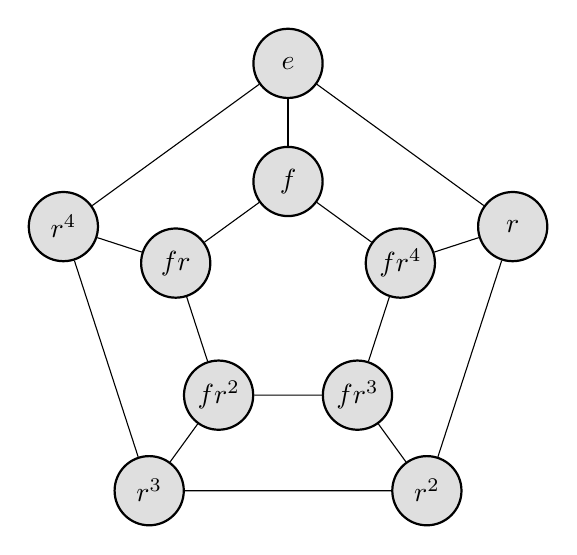
\begin{tikzpicture}[rotate=90,scale=1.5]
\tikzstyle{vertex}=[draw,thick,circle,fill=lightgray!50,minimum size=25pt,inner sep=0pt]
\def\k{360/5}
\draw (-0*\k : 1) node[vertex] (v1)  {$f$};
\draw (-0*\k : 2) node[vertex] (v2)  {$e$};
\draw (-1*\k : 1) node[vertex] (v3)  {$f r^4$};
\draw (-1*\k : 2) node[vertex] (v4)  {$r$};
\draw (-2*\k : 1) node[vertex] (v5)  {$f r^3$};
\draw (-2*\k : 2) node[vertex] (v6)  {$r^2$};
\draw (-3*\k : 1) node[vertex] (v7)  {$f r^2$};
\draw (-3*\k : 2) node[vertex] (v8)  {$r^3$};
\draw (-4*\k : 1) node[vertex] (v9)  {$f r$};
\draw (-4*\k : 2) node[vertex] (v10) {$r^4$};
\draw (v2) -- (v1);
\draw (v2) -- (v1);
\draw (v3) -- (v1);
\draw (v4) -- (v2);
\draw (v4) -- (v3);
\draw (v5) -- (v3);
\draw (v6) -- (v4);
\draw (v6) -- (v5);
\draw (v7) -- (v5);
\draw (v8) -- (v6);
\draw (v8) -- (v7);
\draw (v9) -- (v1);
\draw (v9) -- (v7);
\draw (v10) -- (v2);
\draw (v10) -- (v8);
\draw (v10) -- (v9);
\end{tikzpicture}
\end{comment}

% try to let the text flow to the right of the diagram or: let the diagram appear to the right, or put a few more diagrams  next to each other

% aka Cayley diagrams, Cayley graph,

% https://tikz.dev/tikz-shapes
% https://en.wikipedia.org/wiki/Cayley_graph
% https://beckytikz.wordpress.com/2013/09/21/some-simply-cayley-graphs/  good!
% https://beckytikz.wordpress.com/2013/09/21/cayley-hypergraphs/
% https://graphtheoryinlatex.wordpress.com/
% https://www.sciencedirect.com/science/article/pii/S0012365X12005146

% https://tex.stackexchange.com/questions/222881/cayley-graph-of-free-group-in-tikz

% What's a Cayley map? Embedding of the Cayley graph inot a hypersurface?

%===================================================================================================
\subsection{Conjugacy Classes}
Recall from the linear algebra section the definition of similarity between two matrices. Two matrices $\mathbf{A,B}$ are considered to be similar, denoted by $\mathbf{A} \sim \mathbf{B}$, if there exists an invertible matrix $\mathbf{S}$ such that $\mathbf{B} = \mathbf{S^{-1} A S}$. In group theory there is the notion of \emph{conjugacy} which coincides with the notion of \emph{similarity} when we consider the group of all invertible matrices, i.e. the general linear group. But when we are dealing with a more restricted group of matrices or a group that has nothing to with matrices at all, then the notion of conjugacy becomes a bit more restricted. The equation is the same, though: two group elements $a,b$ are conjugate to one another, if the equation $b = s^{-1} a s$ holds for some $s$ that must also be an element of the group. It is that latter requirement of $s$ being inside the group that makes the notion of conjugacy more restrictive ...TBC...



% https://www.youtube.com/watch?v=vYKdh5oQ4Zw&list=PLi01XoE8jYoi3SgnnGorR_XOW3IcK-TP6&index=8
% 7:40: conjugation can also be applied to a group G or subgroup H or subset A as whole using 
% the notation $B = s^{-1} A s$ 

% $SL_n$

% give algorithm to compute the conjugacy class for a given g \in G

% https://math.stackexchange.com/questions/102170/is-there-a-systematic-way-of-finding-the-conjugacy-class-and-or-centralizer-of-a

% maybe a full subsection is a bit too much for this small topic. Maybe it actually fits into the
% Generators subsection as subsubsection? Is there some connection between generators and 
% conjugacy classes? That seems to be the case indeed:
% https://math.stackexchange.com/questions/397453/finite-group-is-generated-by-a-set-of-representatives-of-conjugacy-classes

% explain: centralizer, normalizer, stabilizer, orbit
% https://en.wikipedia.org/wiki/Centralizer_and_normalizer



% Maybe explain it by way of an example using 2x2 matrices
% Or maybe use a permutation group - maybe S_3. It has 6 elements, so it would be a 6x6
% Cayley table. We need a non-commutative group to demosntrate the concept

% https://en.wikipedia.org/wiki/Conjugacy_class
% https://mathworld.wolfram.com/ConjugacyClass.html
% https://en.wikipedia.org/wiki/Matrix_similarity

%===================================================================================================
\subsection{Subgroups}
If a subset of the underlying set of a group forms itself a group under the same operation, then that subset together with the operation forms what is called a \emph{subgroup} of the original group. As is often the case in mathematical definitions, the edge cases are included in the definitions of terms. A group itself also counts as a subgroup of its own. Also, the group consisting only of the identity element counts as subgroup of any group. These two subgroups always exist for any group and are called the trivial subgroups. A nontrivial subgroup is also called a proper subgroup. The notation for subgroups is as follows: If $S$ is a subgroup of $G$, we write $S \leq G$. In case of $S$ being a proper subgroup, we may also write: $S < G$. In the context of group theory this is not read as "S is less than G" but rather as "S is a subgroup of G".

% https://www.youtube.com/watch?v=KufsL2VgELo&t=1138s
% https://en.wikipedia.org/wiki/Subgroup

\paragraph{Example}
For example, the even integers under addition form a proper subgroup of all the integers under addition. To see this, we just need to verify the group axioms for the even integers: Closure: Sums of even integers are again even - check. Associativity: Inherited from integer addition - check. Neutral element: Zero is among the evens - check. Inverse elements: Negating an even integer gives another even integer - check. Done. The even integers form a subgroup of the integers. The odd numbers, on the other hand, do not form a subgroup of the integers. They fail to contain the neutral element - zero is not odd. They are not even closed under addition: adding two odd numbers gives an even number. Associativity works out fine and inverses are also there - but that's not enough to qualify as a group. 

\medskip
The integers under addition are an infinite group. But we now want to focus on finite groups because many interesting theorems about subgroups are about those finite groups. In a certain way that is analogous to the prime factorization of natural numbers, finite groups can be factored into simpler constituents using a machinery arising from the idea subgroups. Infinity cannot be factorized but this factorization is the thing we are now interested in. Therefore, we'll now focus on finite groups. [TODO: Maybe move this text segment to the "Quotient Groups" section]

\paragraph{Example}
Consider the group $\mathcal{G} = (\mathbb{Z}_{12}, +)$ which we here want to understand as the set of integers modulo $12$ with modular addition modulo $12$ as group operation. Because $12$ has many divisors, $\mathcal{G}$ has quite a lot of (nontrivial) subgroups. You can easily verify that $\{0,2,4,6,8,10\}, \{0,3,6,9\}, \{0,4,8\}, \{0,6\}$ are subgroups of that group. These subgroups are isomorphic to $(\mathbb{Z}_{6}, +)$, $(\mathbb{Z}_{4}, +)$,$(\mathbb{Z}_{3}, +)$, $(\mathbb{Z}_{2}, +)$ respectively. As a general rule, subgroups of cyclic groups are themselves (isomorphic to) cyclic groups. As any group, $\mathcal{G}$ has also the trivial subgroups $\{ 0 \}$ and $\mathbb{Z}_{12}$ itself but we are not interested in them. 

% https://math.stackexchange.com/questions/1718041/list-all-subgroups-of-mathbb-z-6-and-mathbb-z-8
% Maybe use Z_6 instead because we don'T want to use up too much space for the tables.
% It says, that cyclic groups have cyclic subgroups

% https://math.stackexchange.com/questions/208063/calculation-of-subgroups-of-z-12
% https://www.quora.com/How-do-you-find-the-subgroups-of-z12
%It's Cayley table (I don't want to call it multiplication table here) reveals some interesting structure

% maybe use +_{12} - a plus with subscript 12 to denote modular addition...but mayb not

% is (\mathbb{Z}_{12}, +) the same group as in Weitz video - the rotations of the tetraeder?
% https://www.youtube.com/watch?v=UhE0t3SP6E8

% and/or is it isomorphic to D_6, the 12 symmetries of a hexagon?
% https://mathworld.wolfram.com/DihedralGroupD6.html
% https://en.wikipedia.org/wiki/Dihedral_group_of_order_6
% https://en.wikipedia.org/wiki/Dihedral_group

% https://en.wikipedia.org/wiki/Tetrahedral_symmetry

% hmm - no - I don't think so. Z_12 is isomorphic to the group tetrahedron symmetries but D_6 seems to be a different group of order 12. 
% Maybe compute its subgroups, too


% https://www.youtube.com/watch?v=MAcdesa9RqA at around 40:00 he gives a single criterion for showing that something is a subgroup (after that, a similar pair of conditions for subrings)




\paragraph{Langrange's Theorem} If $\mathcal{G}$ is a finite group of order $g$ and $\mathcal{S}$ is a subgroup of  $\mathcal{G}$ of order $s$, then $g$ is a multiple of $s$. [TODO: maybe move down - below discussion of cosets]

% Maybe use |\mathcal{G}| for the order, maybe introduce that notation somewhere earlier

\medskip
In other words, the theorem says that the order of the full group must be divisible by the order of any of its subgroups. This immediately implies that groups of prime order cannot have any nontrivial subgroups because nothing divides a prime (besides itself and one - the trivial divisors). The theorem does not imply that for each divisor of the order group a subgroup exists, though. It should also be noted that there may be more than one subgroup for a given divisor. For example, the alternating group of 4 elements is of order 12 has 3 subgroups of order 2, 4 of order 3, 1 of order 4 and 0 of order 6.

%https://www.youtube.com/watch?v=TCcSZEL_3CQ&list=PLi01XoE8jYoi3SgnnGorR_XOW3IcK-TP6&index=7
% 3:31
% 7:55

%If $\mathcal{S} = (S,\circ)$ is a subgroup of order $|S|$ of a finite group $\mathcal{G} = (G,\circ)$, then the order $|G|$ of $\mathcal{G}$ is a multiple


\subsubsection{Cosets}
A subgroup $H$ partitions its parent group $G$ into equally sized subsets which all have a size of $|G| / |H|$. This partitioning is achieved by picking an element $a$ of $G$ that is not in $H$ and multiplying it by all elements of $H$. For the \emph{left cosets}, the picked element $a$ should be the left factor. That means, after picking $a$ from $G \setminus H$, one forms all possible products $a h$ where $h \in H$. The resulting set of elements is called the left coset of $H$ for the coset representative $a$. Of course, $a$ itself will be in the coset which it represents because $H$, by virtue of being a subgroup, contains the neutral element. The other elements that ended up in the coset can be considered as equivalent to $a$ in the sense of being in an equivalence class with $a$ serving as the representative. It turns out that any other element of the so generated coset, let's call it $a'$, would be just as good as representative. Would we have picked $a'$ instead of $a$, we would have obtained the exact same coset. But there may still be other elements of $G$ that have not yet been generated. Now we pick one of these left over elements, say $b$, and do the same procedure again. Doing so, we will obtain another coset with $b$ as representative. We continue this way until we exhausted the whole group $G$, i.e. have generated all elements of the group and placed each into one of the cosets. The subgroup $H$ itself is also considered to be among its own cosets. In the beginning I said that we should pick $a$ from $G \setminus H$. We could also allow to pick the $a$ from $H$ but in this case, we would just produce the elements of $H$ again. So without the restriction $a \notin H$, the subgroup $H$ would actually fit into the scheme of this coset construction algorithm as an uninteresting edge case where it just reproduces itself. In some sense, the cosets can be considered to be shifted copies of the subgroup $H$. This will be clarified in the example. The notation for the left cosets of some element $g \in G$ with respect to the subgroup $H$ is $g H = \{ g h : h \in H \}$ and the notation for the right cosets is $H g = \{ h g : h \in H \}$.

\paragraph{Example}
Consider the group $\mathbb{Z}_{12} = \{0,1,2,3,4,5,6,7,8,9,10,11\}$ again and let that be our $G$. Let's take the subgroup generated by $\{4\}$ as our $H$. The underlying set of $H$ is given by $\langle 4 \rangle = \{0,4,8\}$ and is as a group isomorphic to $\mathbb{Z}_{3} = \{0,1,2\}$. Now let's pick an element of $\mathbb{Z}_{12}$ which is not in $\langle 4 \rangle$. The first one that occurs is $1$ so let's take that. Now form all possible products of $1$ with elements from $\langle 4 \rangle$ and put them into a set. That gives $\{1+0,1+4,1+8\} = \{1,5,9\}$. That is our first coset with representative $1$. We may also denote this as $1 + \langle 4 \rangle$. There are elements in $\mathbb{Z}_{12}$ which are neither in $H = 0 + \langle 4 \rangle$ nor in $1 + \langle 4 \rangle$, so we pick one of these leftovers. The first possibility is $2$, so we pick that. Repeating the procedure, we obtain $2 + \langle 4 \rangle = \{2,6,10\}$. We have still not exhausted $G$ so we do one more round to obtain a 4th coset given by $3 + \langle 4 \rangle = \{3,7,11\}$. So, in summary, our procedure generated the 4 cosets $0 + \langle 4 \rangle = \{0,4,8\}$, $1 + \langle 4 \rangle = \{1,5,9\}$, $2 + \langle 4 \rangle = \{2,6,10\}$, $3 + \langle 4 \rangle = \{3,7,11\}$. These are 4 cosets of size 3 and $4 \cdot 3 = 12$ which is the size of our group $G$ as it should be. Looking at the numbers, we see that they are all shifted copies of $\{0,4,8\}$ where the shift amount is given by the element of $G$ that is added from the left. You may verify yourself that, due to the behavior of modular addition, we would have arrived at the same cosets if we would have chosen other representatives. For example, the coset $\{1,5,9\}$ could also have been obtained as $5 + \langle 4 \rangle$ or $9 + \langle 4 \rangle$. The elements would have been obtained in a different order but at the end, it would be the same collection of elements - and order doesn't matter in a set. In this specific example, we would also have obtained the same sets if we had formed the right cosets instead of the left ones, i.e. $\langle 4 \rangle + 1$ instead of $1 + \langle 4 \rangle$ etc. This is so because our example group is commutative. In general, this doesn't need to be the case. In general left cosets and right cosets may be different.

\paragraph{}
The takeaway is that a subgroup $H$ always partitions a group $G$ into equally sized equivalence classes of elements which we call (left or right) cosets with respect to the subgroup $H$. The different cosets cannot have common elements, i.e. two different cosets are always disjoint. The number of cosets that $H$ generates in $G$ is called the \emph{index of $H$ in $G$} and denoted as $|G : H|$. We will always have $|G| = |H| \cdot |G : H|$. The cosets can be considered to be equivalence classes. Their elements are equivalent in the sense that each of them would give rise to the same coset when being picked in our construction algorithm. The elements that are bunched together into one coset are considered to be equivalent by an equivalence relation which we denote by $\equiv$, i.e. $x \equiv y$ means: "$x$ is equivalent to $y$" in the sense of "$x$ and $y$ are in the same coset". In the example, we have $0 \equiv 4 \equiv 8$, $1 \equiv 5 \equiv 9$, $2 \equiv 6 \equiv 10$ and $3 \equiv 7 \equiv 11$. If we are given two elements $x,y$ of $G$ and we want to figure out whether or not $x \equiv y$, we note that this equivalence happens whenever $y = x h$ for some $h \in H$. Therefore, we may form $x^{-1} y = h$ and check if the result $h$ can be found in $H$. If so, then yes indeed: $x \equiv y$, otherwise not. If we are given one element $x \in G$ and want to figure out into which coset it belongs, we compare it via $\equiv$ to a representative of each of the cosets in turn. As soon as $\equiv$ reports "yes", we have found our coset into which $x$ belongs [VERIFY! see comment in .tex file].



% ToDo: maybe use the \equiv symbol for the equivalence realtion defined here, see:
% https://www.geeksforgeeks.org/equality-and-inference-symbols-in-latex/
% I think this would also be consistent with the notation used in modular arithmetic for 
% congruence. 
% https://en.wikipedia.org/wiki/Modular_arithmetic
% There is also a "congruent to" symbol \cong but that's maybe not suitable
% We may then use \sim for similarity in the sense of being in the same conjugacy class.

% ToDo: give an example calculation. To do this, we may also need the list of inverse elements in Z_12 which is given by:
%
% x:     0  1  2  3  4  5  6  7  8  9 10 11
% x^-1:  0 11 10  9  8  7  6  5  4  3  2  1
%
% to check that 5 and 9 are equivalent, the comutation is:
%
% 5 ~ 9   bcs  5^-1 * 9 = 7 * 9 = 16 = 4 (mod 12)  which is in H = {0,4,8}
%
% note that the * here actually stands for modular addition and 5^-1 for the additive modular inverse of 5 in Z_12 which is 7. It's a bit confusing. In the text, we'd use juxtaposition

% Explain how we can interpret the set of cosets as a group and how we can calculuate with these cosets. If we just pick the first element from each coset, we get {0,1,2,3}. Should we interpret that as Z_4? But what if we pick other representatives? Maybe it still works but we need to pick the "corresponding" representatives like 4,5,6,7 or 8,9,10,11? But how can we formalize this correspondence? 

% Or maybe we take the whole cosets as elements of our new group. Maybe the new group could be made from {{0,4,8},{1,5,9},{2,6,10},{3,7,11}} and the group operation works like {1,5,9} * {2,6,10} = {3,7,11}. But how do we figure out the new multiplication table? Maybe that has to be done already during the construction of the cosets and can't be inferred from the cosets alone after the fact?

% It's explained in Riley et al, pg 1065ff and works as follows:
% We have x ~ y if x^{-1} y is in H because this is the same as saying y = x h for some h in H, So, to test if x and y are equivalent, we need to fom x^{-1} y and check whether or not the result is an element of H. I think, to calculate with the cosets, we can pick an arbitrary element from each of the cosets and then do our calculations with that set of picked elements. Each element represents its coset. I guess, the computations could sometimes spit out other elements from the cosets, i.e. not always produce our chosen representants. But we can just continue computing - if this happens, we have just swapped the representative within the computation which doesn't matter. at te very end of the computation, we may map the final result back to its representative by looking in which of the classes the result ended up in

% I'm not totally sure about that and have not yet tried it thoroughly.

% Maybe in practice, one could built a multiplication table for the cosets during the construction of the cosets 


\subsubsection{Special Subgroups}
Not all subgroups are created equal. There are certain special types of subgroups that are important enough to deserve special names.

\paragraph{Normal Subgroups} The textbook definition of a \emph{normal subgroup} is:  A subgroup $N$ is called normal, iff $g^{-1} N g = N$ for any $g \in G$. In words, this may be stated as: normal subgroups are invariant under conjugation. If this is the case, then the cosets of $N$ form themselves a group. This group is, in general, not a subgroup of $G$ (TODO: Is it ever? Figure out!). The group of cosets is called a \emph{factor group} or \emph{quotient group} and denoted as $G / N$. It has $N$ as the identity element and the inverse of $g N$ is $g^{-1} N$ for any $g \in G$ [VERIFY]. Another equivalent way to characterize normal subgroups is to say their left and right cosets coincide. The notation for normal subgroups is $N \triangleleft G$. [TODO: list more equivalent ways to characterize a normal subgroup - see wikipedia]

\medskip
A subgroup $H$ of some group $G$ may itself not be a normal subgroup of $G$ but it may contain smaller subgroups that are normal subgroups of $G$. The largest of those is called the \emph{normal core} of $H$. If $H$ is already a normal subgroup, then its normal core is $H$ itself, of course.

% maybe mention p-cores

%...TBC...
% https://en.wikipedia.org/wiki/Normal_subgroup
% https://en.wikipedia.org/wiki/Normal_subgroup#Equivalent_conditions
%  -> the communtator of every n in N and g in G is in N

% https://www.youtube.com/watch?v=vYKdh5oQ4Zw&list=PLi01XoE8jYoi3SgnnGorR_XOW3IcK-TP6&index=8
% 8:29: A subgroup $N$ is normal, iff $g^{-1} N g = N$ for any $g \in G$
% If this is the case, then the cosets of $N$ form themselves a group (which is not a subgroup 
% of $G$ in general...is it ever?). The group of cosets is called a factor group and denoted as
% $G / N$. It has $N$ as the identity element and the inverse of $x N$ is $x^{-1} N$

% Notation < for subgroups and the triangle for normal subgroups

% https://en.wikipedia.org/wiki/Core_(group_theory)
% https://en.wikipedia.org/wiki/P-group

\paragraph{Commutator Subgroup} The commutator subgroup of a group $G$ is the subgroup generated by all of its commutators. A \emph{commutator} $c$ of a group $G$ is an element that is generated from two elements $a,b$ via the commutator operation $[a,b] = a^{-1} b^{-1} a b$. If and only if $a$ and $b$ commute, i.e. iff $ab = ba$, then their commutator will be the identity element $e$. If they don't commute, then it will be some other element. Now we can produce the set of all possible commutators. In general, this will give a subset of $G$ which is not necessarily a subgroup. But if we use this subset as generator, we will get a subgroup and that group is called the commutator subgroup. A group that is equal to it own commutator subgroup, i.e. a group that can be fully generated by the set of its commutators, is called a \emph{perfect group}.


[TODO: explain relation to matrix commutator $\mathbf{AB - BA}$ - there seems to be potential for confusion - it's clearly a different operation with the same name]

% https://en.wikipedia.org/wiki/Commutator_subgroup
% https://en.wikipedia.org/wiki/Commutator
% https://en.wikipedia.org/wiki/Perfect_group

% Maybe say more about perfect groups, see wikipedia article
% -they have no nontrivial commutative quotient groups

%\paragraph{Torsion Subgroup}
% https://en.wikipedia.org/wiki/Torsion_subgroup
% applies to infinite groups - not sure if it belongs here

\paragraph{Center of a Group}
The \emph{center} of a group $G$ is the set of elements that commute with every element of $G$. If the center consists only of the identity element, which always trivially commutes with everything, the group is called \emph{centerless}. The center of a group is always a commutative normal subgroup. The elements of the center are sometimes called \emph{central}.

% https://en.wikipedia.org/wiki/Center_(group_theory)

%\paragraph{Centralizer and Normalizer}
% https://en.wikipedia.org/wiki/Centralizer_and_normalizer
% https://math.stackexchange.com/questions/1334437/difference-between-centralizer-and-center-groups

%\paragraph{Characteristic Subgroup}
%The commutator and center subgroups are examples of so called characteristic subgroups.
% https://en.wikipedia.org/wiki/Characteristic_subgroup
% https://en.wikipedia.org/wiki/Automorphism
% https://en.wikipedia.org/wiki/Free_group

\subsubsection{Product Groups}
% https://en.wikipedia.org/wiki/Direct_product_of_groups
% https://en.wikipedia.org/wiki/Semidirect_product
% https://en.wikipedia.org/wiki/Zappa%E2%80%93Sz%C3%A9p_product
% https://en.wikipedia.org/wiki/Wreath_product


% https://en.wikipedia.org/wiki/Klein_four-group
% is direct product Z_2 x Z_2

% https://en.wikipedia.org/wiki/List_of_small_groups

% https://www.youtube.com/watch?v=rXLz8TdckWo&list=PLi01XoE8jYoi3SgnnGorR_XOW3IcK-TP6&index=21
% Not all non-simple finite groups can be made via the direct product. It's more complicated.

\subsubsection{Quotient Groups}
We are now interested in how we can break down certain groups into smaller constituent groups. To see how this could work, we will first consider the opposite: how can we build a larger group from two smaller constituent groups?

% https://www.youtube.com/watch?v=vYKdh5oQ4Zw&list=PLi01XoE8jYoi3SgnnGorR_XOW3IcK-TP6&index=8
% 3:59: "the cosets form a group" ... called the quotient group....a coset group. This group is
% NOT a subgroup of the original group! Cosets wrt a subgroup H will only form a group if H is a
% normal subgroup

% https://www.youtube.com/watch?v=vYKdh5oQ4Zw&list=PLi01XoE8jYoi3SgnnGorR_XOW3IcK-TP6&index=8
% 10:25 Normal subgroups and quotient groups ar among the most useful devices in abstract algebra.
% It  also say something about "Composition Series"

% https://en.wikipedia.org/wiki/Coset
% Cosets of normal subgroups can be used as elements of another group (how?), called the quotient group

\subsubsection{Composition Series}
% A kind of prime factorization of the group

% https://www.youtube.com/watch?v=jhVMBXl5jTA&list=PLi01XoE8jYoi3SgnnGorR_XOW3IcK-TP6&index=22

% How does the "construction" of non-simple finite groups work? Is it based on the cartesian product of the underlying sets where the individual group operations are applied element-wise? add a segment under the "Subgroups" section, mabye name it "Group Factorization" - look up, how it's called and how it's done

% Maybe relevant:
% https://en.wikipedia.org/wiki/Quotient_group
% https://mathworld.wolfram.com/QuotientGroup.html
% https://en.wikipedia.org/wiki/Group_extension
% https://feog.github.io/lecture9ws.pdf
% https://www.math3ma.com/blog/whats-a-quotient-group-really-part-1
% https://math.stackexchange.com/questions/625433/what-does-factorization-of-a-group-mean
% https://en.wikipedia.org/wiki/Algebraic-group_factorisation_algorithm
% https://en.wikipedia.org/wiki/Direct_product_of_groups
% https://en.wikipedia.org/wiki/Semidirect_product
% https://www.youtube.com/watch?v=KufsL2VgELo at 25:40
%https://en.wikipedia.org/wiki/Composition_series#For_groups





\subsection{Morphisms (Iso-, Homo- and more)}

% Maybe this should go before the subsection about subgroups because automorphisms are referenced there. But no - a theorem stated here requires the notion of a normal subgroup. We have a cross-referencing problem here

Morphisms in group theory are functions $f$ that map from the underlying set of one group to the underlying set of another group. In group theory, you don't commonly encounter the term morphism all by itself. It's usually prefixed by some qualifier because we are mostly interested in functions that satisfy certain constraints. The most important specimen are \emph{isomorphisms} and \emph{homomorphisms}. There are also \emph{epimorphisms}, \emph{monomorphisms} and \emph{automorphisms}. Let's see what they are.

\subsubsection{Homomorphisms}

Assume we have a group $\mathcal{G} = (G, \circ)$ and another group $\mathcal{H} = (H, \diamond)$. Assume furthermore that we have a function $f: G \rightarrow H$ that maps elements from $G$ to elements from $H$. That function is called a group homomorphism from $G$ to $H$ if it has the following property for all $a,b \in G$:
\begin{equation}
	f(a \circ b) = f(a) \diamond f(b)
\end{equation}
This equation says that it doesn't matter whether we firstly combine $a$ and $b$ in $G$ via $\circ$ and then secondly map the result over to $H$ via $f$ or if we firstly map $a$ and $b$ separately over to $H$ via $f$ and then secondly combine them over there via $\diamond$. The end result should be the same in both cases. Such a function $f$ is constrained to preserve the structure of group $G$ while mapping over to group $H$ and it may or may not exist. If such a homomorphism does exist then we can find the structure of group $G$ within group $H$ in the sense that the image of $G$ is a subgroup of $H$. Note that, as promised, I'm sloppy with using $G$ and $H$ as stand-in in some places where it would actually be more correct to write $\mathcal{G}$ and $\mathcal{H}$. Formally, it makes no sense to talk about a subgroup of $H$ because $H$ is just a set and the group is actually the pair $\mathcal{H}$. But to state that stuff formally correctly would be very awkward and confusing. Formally correctly, one would have to say that $f$ maps $G$ to a subset of $H$ and that subset happens to be the underlying set of a subgroup of $\mathcal{H}$. Nobody wants to speak like that so this slight sloppiness is quite common and acceptable in group theory [VERIFY!]. Anyway - the essence of a homomorphism is that the function $f$ maps from $G$ to $H$ and thereby preserves the structure of $\mathcal{G}$ within $\mathcal{H}$ - and such a thing may or may not be possible for two given groups at hand. If it is possible, then we may say that $\mathcal{H}$ is homomorphic to $\mathcal{G}$ which means that we find the structure of $\mathcal{G}$ within $\mathcal{H}$ [VERIFY!].

\paragraph{Example}
Let  $\mathcal{G} = (\mathbb{R}, +), \; \mathcal{H} = (\mathbb{R}^+, \cdot)$ and $f: \mathbb{R} \rightarrow \mathbb{R}^+$ with $f(x) = e^x$. That is, we consider the exponential function as a map from the real numbers with addition to the positive real numbers with multiplication. It is indeed a homomorphism between these two groups because $e^{a+b} = e^a \cdot e^b$ for all $a,b \in \mathbb{R}$. On the left hand side, we first add $a$ and $b$ (adding is the group operation of $\mathcal{G}$) and then map the sum over via $f$. On the right hand side, we first map $a$ and $b$ over seperately via $f$ and then multiply (multiplication is the group operation of $\mathcal{H}$). As we know from the laws of exponential functions, the result is the same, so $f$ is indeed a homomorphism.

% maybe say something about the logarithm as inverse homomorphism...but maybe later
% verify that neutral and inverse elements get mapped to their counterparts

% Riley/Hobson et al pg 1060 use the complex exponential as example for an isomorphism. mayb do that, too

% https://www.youtube.com/watch?v=XPF5fe1WdKY&list=PLi01XoE8jYoi3SgnnGorR_XOW3IcK-TP6&index=11
% Has another example: Z and Z_2 the homomorphism maps the evens to 0 and the odds to 1
% also: (Z_4,+) and({1,i,-1,i},*)

\paragraph{} Homomorphisms have some noteworthy properties. To state them, we first need another definition: The \emph{kernel} of $f$ is the set of elements of $G$ that are mapped by $f$ to the neutral element $e_H$ of $H$: $\ker(f) = \{ k \in G: f(k) = e_H \}$. In other words, the kernel of $f$ is the pre-image of the neutral element in $H$. Now we can say that: (1) The image of $G$ under $f$ is a subgroup of $H$. (2)  The kernel of $f$ is a normal subgroup of $G$.

% Make this theorem look more important bcs it is (I think)

%https://mathworld.wolfram.com/GroupHomomorphism.html

% https://www.youtube.com/watch?v=TngePpJ_x-I&list=PLi01XoE8jYoi3SgnnGorR_XOW3IcK-TP6&index=14
% The kernel of f measures how much bigger G is? But no! It's a property of f - not of G,H. The
% kernel measures to which degree f fails to be 1-to-1. If the kernel only contains the identity,
% then f is 1-to-1

\subsection{Isomorphisms}
Isomorphisms are homomorphisms that satisfy some additional constraints. These are: (1) Different elements of $G$ must be mapped to different elements of $H$. That is: $f$ must be injective. (2) Every element of $H$ must be reached by $f$. That is: $f$ must be surjective. Taken together, these two additional requirements require $f$ to be bijective and therefore invertible. Therefore, an isomorphism is a homomorphism that works in both directions. That means: mapping from $G$ to $H$ preserves the structure of $G$ in $H$ and mapping back from $H$ to $G$ preserves the structure of $H$ in $G$. Again, an isomorphism between two given groups may or may not exist. If one does exist, we may say that the two groups are isomorphic which means: of equal form \footnote{The internet says that "iso" means "equal" whereas "homo" means "the same" - and there is supposed to be a subtle difference. But it actually says that the difference is such that "homo" should be the stronger form (identity) and "iso" the weaker form (equivalence) - but here it's clearly the other way around: iso is the stronger form of sameness-morphism than homo. I don't know what to make of that. It's a mess!}. If two groups are isomorphic, they are structurally the same. One is actually the other in disguise and vice versa in the sense that the elements of the underlying sets are just "renamed" with respect to one another via $f$. 
That's why isomorphisms are so important in group theory. They are a tool to convince ourselves that two superficially very different mathematical setups are actually in some sense the same such that we can transfer knowlegde obtained in one domain to the other. Or even better: abstract out the commonalities explicitly, as we do in abstract algebra.
% Was our homomorpism above actually an isomorphism? What about injecting the inamginary unit itno the expoenent? I think, then it becomes a homo- but not isomorphism (see Riley, Hobson et. al., page 1060)

\paragraph{}
\emph{Isomorphisms} are the most important kind of morphisms in group theory, followed by \emph{homomorphisms} [my personal judgement - VERIFY]. There are also \emph{monomorphisms} which are injective homomorphisms and \emph{epimorphisms} which are surjective homomorphisms. They are somewhere in between the homomorphisms and isomorphisms in terms of how constrained they are. An \emph{automorphism} is an isomorphism from a group to itself.

% https://en.wikipedia.org/wiki/Automorphism
% https://en.wikipedia.org/wiki/Automorphism_group





%===================================================================================================
\subsection{Representation Theory}
A group is abstractly defined as a set on which a binary operation is defined that satisfies certain properties. The elements of the set can be anything. Fortunately, there is a generic way for how we may concretely represent elements of a group and also a generic way to implement its group operation. Each group element is represented by an invertible matrix and the group operation is mapped to matrix multiplication. We have already mentioned that the set of symmetries of a regular polygon can be represented by a specific set of $2 \times 2$ matrices, see (\ref{Eq:PolygonSymmetries}). Such a representation of the group as a set of matrices is possible for any group whatsoever [VERIFY!]. ...TBC...


% https://en.wikipedia.org/wiki/Representation_theory
% https://en.wikipedia.org/wiki/Group_representation
% https://en.wikipedia.org/wiki/Representation_theory_of_finite_groups

% ToDo: give a representation of (Z,+) via matrices. We may need to use homogeneous coordinates and/or the logarithm

% Is it possible to faithful represent any group via matrices?
% https://en.wikipedia.org/wiki/Representation_theorem

%===================================================================================================
\subsection{Taxonomy of Groups}

% ToDo: Cyclic, Abelian, Alternating, Symmetric, Dihedral, Coxeter
% and this text here should go as subsubsection into it

\subsubsection{Permutation Groups}
A \emph{permutation} of a finite set $A = \{ 1,2,\ldots,n \}$ with $n$ elements is an arrangement of its elements. Sets themselves do not have any notion of order, so we denote such an arrangement of the $n$ elements in the form of an $n$-tuple. Let's take the set $A = \{ 1,2,3 \}$ and assume its natural order is $(1,2,3)$. The set of all possible arrangement of these $3$ elements in a tuple is given by $\{ (1,2,3), (1,3,2), (2,1,3), (2,3,1), (3,1,2), (3,2,1) \}$. These are all the possible $6$ arrangements or permutations of $3$ objects. In general, there are $n!$ different ways to order $n$ objects.

[TODO: introduce notation for permutations]...TBC...

% https://en.wikipedia.org/wiki/Permutation

\paragraph{Transpositions and Parity}
Given a tuple $x = (x_1, x_2, \ldots, x_n)$ we call the act of swapping two elements in this tuple a \emph{transposition}. It turns out that the set of all possible permutations can be partitioned into those that can be achieved only with an even number of transpositions and those that can be achieved only with an odd number of transpositions. We call the former permutations \emph{even} and the latter permutations \emph{odd}. This evenness vs oddness feature of a permutation is called \emph{parity}.

% Tranposition = Swap
% https://en.wikipedia.org/wiki/Cyclic_permutation#Transpositions

\paragraph{Decomposition into Cycles}
Any permutation can be decomposed into simpler constituents which are called \emph{cycles}. This works as follows....TBC...

% a transposition is a 2-cycle 
% these cycles do not interact with one another, i.e. each cycle operates on its own a set of 
% indices with no overlap with any of the other cycles. Therefore, it doesn't make any difference
% in which order we apply two successive cycles - i.e. the cycles commute.
% Of course, this has nothing to do with the question whether or not the permutations themselves
% commute - in general, they will not. It also doesn't say that one cycle from a permutaion P1
% commutes with one cycle from another permutation. These cycles are inner sub-permutations within
% one single permutation. I think, two permutation will generally commute, iff they operate on 
% different index sets. ...Or maybe that's a sufficient but not necessarry condition? Two 
% permutations that are inverses of each other also commute but operate on the same index set.
% Maybe their permuations matrices must be symmetric?

\paragraph{Cayley's Theorem} Every group is isomorphic to a subgroup of a symmetric group.

\medskip
This theorem is important because it allows us to have a more concrete picture in our mind when thinking about groups. ...TBC...

% https://en.wikipedia.org/wiki/Cayley%27s_theorem

% Be more concrete - the theorem states more about how these subgroups look like

%---------------------------------------------------------------------------------------------------
\subsubsection{Lie Groups}
A Lie group is a group, whose underlying set may be interpreted as a set of points that live on a \emph{manifold}. For example, the set of all rotations of the 2D plane may be interpreted as points on the unit circle. The unit circle is a curve, i.e. a 1D manifold that we usually envision to live in a 2D embedding space. We can identify points on the unit circle with rotation angles. This group is also called the \emph{circle group} and sometimes also the \emph{special orthogonal group} of order 2 and denoted by $SO(2)$. In a matrix representation of an orthogonal group, all matrices will have a determinant of $\pm 1$ and in a special orthogonal group, they will only have determinant $1$. Orthogonal means that the matrices encode orthogonal transformations which are a combination of rotations and reflections. In the "special" ones, only rotations are allowed. This group of 2D rotations can also be represented by complex numbers of unit modulus where complex multiplication serves as group operation, i.e. encodes the composition of the rotations. Note that in the representation via complex numbers, the associated manifold, namely the circle, naturally emerges as a curve in the plane. In a matrix representation, however, it might seem like the manifold lives in a 4D space because general $2 \times 2$ matrices have 4 entries. However, a manifold all by itself does not need to be thought of as being embedded into some higher dimensional space. We can also take an intrinsic point of view in which the manifold is just characterized by its own intrinsic dimensionality, which is 1 in this case, without reference to any embedding space. This should remind us of things like intrinsic curvature in differential geometry. The embedding space is just a tool for us to visualize the manifold. More generally, we may consider the groups of rotations in an $n$D space. They are called the special orthogonal groups of order $n$ and denoted by $SO(n)$. 

%https://en.wikipedia.org/wiki/Quotient_group#The_real_numbers_modulo_the_integers
% The circle group is isomorphic to R \ Z

%Topologically, these groups form an $n$-torus which means ...well...nope
% SO(2) is topologically a 1-torus and generally SO(n) is an n-torus

% Lie groups are at the intersection of group theory, linear algebra and differential geometry.
...TBC...

%For example, the set of all rotations in 3D may be interpreted as the surface of the unit sphere [VERIFY!]. ...nope! SO(3) is 3D, says wikipedia. A point on a sphere can't encode any rotation around an axis that goes through the point. But could the unit sphere encode some other intersting set of transformations? Or maybe a torus? I think, they may encode rotations in a given plane, say, the xy-plane. ...ah - no - for this, 1 number is sufficient..soo maybe rotations around 2 axes but not all 3?

% https://en.wikipedia.org/wiki/Lie_group
% https://de.wikipedia.org/wiki/Lie-Gruppe
% https://mathworld.wolfram.com/LieGroup.html
% https://en.wikipedia.org/wiki/Table_of_Lie_groups
% https://en.wikipedia.org/wiki/Simple_Lie_group
% https://en.wikipedia.org/wiki/Representation_of_a_Lie_group
% https://en.wikipedia.org/wiki/Lie_algebra_representation
% https://en.wikipedia.org/wiki/Circle_group
% https://en.wikipedia.org/wiki/3D_rotation_group
% https://en.wikipedia.org/wiki/Orthogonal_group
% https://en.wikipedia.org/wiki/Orthogonal_group#Special_orthogonal_group
% https://en.wikipedia.org/wiki/Poincar%C3%A9_group
% https://en.wikipedia.org/wiki/Quaternion_group
% https://en.wikipedia.org/wiki/List_of_small_groups
% https://en.wikipedia.org/wiki/Klein_four-group
% https://en.wikipedia.org/wiki/Dihedral_group

% https://en.wikipedia.org/wiki/Dihedral_group_of_order_6 
% = Z_3 * Z_2, symmetries of triangle, smallest non-abelian, equals S_3

% -Give examples of Lie groups
%  -simple construction: take an existing continuous Lie group and replace R with a finite field
%    ...does it work like that? I'm not sure.
%  -Explain E_8
% -Say something about Lie algebras...or maybe defer that to a chapter about Algebras

\subsubsection{Classification of Finite Groups}
One of the great achievements of modern mathematics is the classification of all finite groups. We have something like a periodic table (as in chemistry) for groups. Another analogy could be the prime numbers - all natural numbers greater than one can be "built" multiplicatively from these prime numbers [TODO: elaborate this "build" process for groups]. Similarly, all groups can be constructed from a known pool of elementary groups which are called the \emph{simple groups} in this context. Simple means that they can't be broken down any further into smaller groups, i.e. have no nontrivial normal subgroups - but they may actually be quite complicated indeed. Let's state the theorem:

\paragraph{Classification Theorem}
Every finite simple group is isomorphic to one of the following groups:
\begin{itemize}
\item A \emph{cyclic group} of prime order.
\item An \emph{alternating group} of degree at least $5$.
\item A group of the \emph{Lie type}.
\item One of 27 of the so called \emph{sporadic} groups.
\end{itemize}
% Theorem from Weitz video at 1:46

The first 3 items describe infinite families of groups whereas the last item, the sporadic groups, are outliers that do not fit into any of the systematic ways to construct groups. Let's now have a look at what kind of groups these classes entail.

\paragraph{Cyclic Groups}
The cyclic groups are named like that because they generate all their elements from repeatedly applying a single generator. After all elements have been generated, they cycle back to the initial element - at least when the group is finite. In the framework of interpreting group members as actions, we can think of the finite cyclic groups as encoding the rotational symmetries of regular polygons. The generator would be the basic rotation around some angle of which all the other rotation angles are integer multiples. For example, all rotations of the regular pentagon that leave it unchanged have angles that are a multiples of 72 degrees. Repeatedly applying a 72 degree rotation 5 times yields a 360 degree rotation which is the same as a 0 degree rotation which is the neutral element. Applying it once more, we are back at the  72 degree rotation again, i.e. we have cycled through all possible rotations are ar now back at our initial rotation angle. We could also have used another element as generator. Repeatedly applying a 144 (= $72 \cdot 2$) degree rotation will also hit the neutral element after 5 repetitions and applying it once more cycles back to 144 again. We can also think of the cyclic groups in terms of modular addition. The group $(\mathbb{Z}_5, +)$ is essentially the same group, i.e. it is isomorphic to the group of rotations by multiples of 72 degrees. All cyclic groups of order $p$ can be represented by $(\mathbb{Z}_p, +)$. Of course, we could also use a set of $2 \times 2$ matrices with matrix multiplication for a concrete representation. When $p$ is a prime, then the group is simple because it cannot possibly have any nontrivial subgroups, much less normal subgroups due Lagrange's theorem. The cyclic groups are commutative and they are the only simple groups with that property. That means: every simple commutative group is cyclic and every non-cyclic commutative group isn't simple. The cyclic group of order $p$ is also denoted as $Z_p$ and its order is given by $p$. 

% Give notation - I think, it's $C_n$. Order of the cyclic group is equal $n$
%

\medskip
Infinite groups such as $\mathbb{Z}$ may also be called "cyclic". The criterion is to be generated by a single generator and $\mathbb{Z}$ can be generated by $\{1\}$ or $\{-1\}$. The \emph{fundamental theorem of finitely generated commutative groups} says that any such group can be broken down to a finite number of cyclic groups.

% https://www.youtube.com/watch?v=8A84sA1YuPw&list=PLi01XoE8jYoi3SgnnGorR_XOW3IcK-TP6&index=9
% 4:09: the fundamental theorem of finitely generated abelian groups
% I think, what she says is that any infinite cyclic group is isomorphic to the integers

% Finite cyclic groups repeat themselves inc cylces. that's where the name comes from

%  Maybe consider the rotations of a hexagon and explain, how this group can be factored


%\paragraph{Dihedral Groups}
% Symmetries of an n-sided polygon. There are $2n$ of them - $n$ rotations and $n$ reflections. Not commutative. Notations: $D_n, D_{2n}$


%\paragraph{Symmetric Groups}

% https://www.youtube.com/watch?v=3aNeCWRjh8I&list=PLi01XoE8jYoi3SgnnGorR_XOW3IcK-TP6&index=16
% Every finite group is a subgroup of a symmetric group (Cayley's Theorem)

% https://www.youtube.com/watch?v=MpKG6FmcIHk&list=PLi01XoE8jYoi3SgnnGorR_XOW3IcK-TP6&index=17
% Cycle notation

\paragraph{Alternating Groups}
Recall that the set of all permutations of $n$ objects forms a group which is called the symmetric group of order $n$ and is denoted by $S_n$. These symmetric groups have as normal subgroup the set of all even permutations, i.e. the set of all permutations that can be achieved by an even number of swaps ("transpositions"). This subgroup of some given $S_n$ is called the alternating group and denoted by $A_n$. If $n \geq 5$, then $A_n$ is simple. This is related to the fact that for polynomials of degree $d \geq 5$ no closed form formulas exist for the zeros. The order of $A_n$ is given by $|A_n| = \frac{n !}{2}$. $A_5$ is the smallest non-commutative simple group and has 60 elements.

% explain the relation to the nonexistence of formulas some more.




\paragraph{Groups of the Lie Type} This is a big family with a lot of subfamilies...TBC...
% should not to be confused with Lie groups?
% They aris from Lie groups in some way of discretizing them?

% https://en.wikipedia.org/wiki/Group_of_Lie_type

\paragraph{Sporadic Groups}

% https://en.wikipedia.org/wiki/Sporadic_group
% https://en.wikipedia.org/wiki/Tits_group

% One of the sporadic groups is so special that some authors do not include it into the class of sporadic groups but rather think of it as being solitarily in a class of its own. That group is the Tits group. I take the stance that if something doesn't even fit into the sporadic groups then it is in some sense extra-sporadic and therefore certainly qualifies as sporadic. 

% Tits group is sometimes not included into the set of sporadic groups. It sits somewhere in between being sporadic and being of Lie type

% https://www.youtube.com/watch?v=jhVMBXl5jTA&list=PLi01XoE8jYoi3SgnnGorR_XOW3IcK-TP6&index=22
% monster group contains 20 of the sporadic groups as subgroups or quotient groups. These are 
% known as the "happy family". The remaining ones are called the "pariahs"


% https://en.wikipedia.org/wiki/Classification_of_finite_simple_groups
% https://en.wikipedia.org/wiki/List_of_finite_simple_groups
% https://en.wikipedia.org/wiki/Group_of_Lie_type

% Weitz:
% https://www.youtube.com/watch?v=UhE0t3SP6E8

% https://en.wikipedia.org/wiki/Finitely_generated_abelian_group
% about classification of finitely generated groups...next step in the classification?



\begin{comment}

https://en.wikipedia.org/wiki/Group_(mathematics)
https://en.wikipedia.org/wiki/Cayley_table
https://en.wikipedia.org/wiki/Dihedral_group
https://en.wikipedia.org/wiki/Group_action
https://en.wikipedia.org/wiki/Category:Theorems_in_group_theory

ToDo:

-Group Visualization (Caley Graphs)
 https://en.wikipedia.org/wiki/Cayley_graph
-Group "Presentation"?
-Give generator and some defining equations instead of the full table. Is that the 
 "presentation"?
 https://en.wikipedia.org/wiki/Presentation_of_a_group
 https://math.stackexchange.com/questions/1401895/finding-the-number-of-defining-equations-of-a-group
-Solving equations in groups
 -single equations, simulatneous equations in one and in multiple variables

Cayley's theorem:
Every group $(G, \circ)$ is isomorphic to a subgroup of the symmetric group $S_G$ of $G$. Here, $S_G$ is the group of all permutations on the set $G$, i.e. the group of all bijective functions from $G$ to $G$.
https://www.youtube.com/watch?v=diLuZiXfdUI&list=PLb0zKSynM2PCLnXVwfjVcefXa6iZA-an4&index=28

Ideas:
-Algorithm to find the subgroups of a given finite group G
 -take an element a form the group and repeatedly apply the group operation to a with itself,
  i.e. produce the powers of a: a^1,a^2,a^3, .... At some point, we will hit the neutral 
  element and after that cycle back to a. 
 -all the elements that were generated from a (commutative) subgroup of G. It must be
  commutative because writing out the powers just gives a long string of a - like 
  a^5 = a a a a a. Obviously, the order in which we write the as doesn't matter because it's 
  all just as anyway.
 -If any elements from the group were not hit by the powers of a, select one of the leftovers
  and repeat the same process with that. that should generate another subgroup.
 -Repeat that until nothing is left over. that should find all subgroups.
-Algorithm for factoring a finite group G:
 -Input should be a Cayley table, output an array of Cayley tables.
 -Find the subgroups of G via the algo above and find their Cayley tables.
-Algorithm for "multiplying" two groups, given their Cayley tables
 -Input is a pair of Cayley tables, output a single Cayley table
 -I think, we need to form something like the Kronecker product of the matrices? Each element
  of one table should give rise to a block in the combined table by being multiplied with an
  element from the other table...or something....not quite sure
  ...after that, we may or may not want to reorder the table..but maybe not - it seems more
  natural to leave it like that...but maybe with the reordering, we could make the operation
  of cobining tables commutative which kight be desirable. How could such an ordering look 
  like? the first row and column should always list the lements in natural order because it's
  the row/col of the neutral element. Maybe we could say that the next row/col should be in 
  ascending order (execpt maybe for the first element)? Is that enough to uniquely determine 
  an order? Figure out! If not, maybe  the third row, or at least part of it (maybe except the
  first two elements), should be ordered too...and so on? Maybe that ordering algorithm could 
  then also be used to check two tables of isomorphy - just order them both and then compare 
  for equality. We would establish a canonical form of Cayley tables.
 -The algo can be used to combine more that 2 tables by taking the result of one application
  as input to the next iteration, i.e. we "fold" the array of input tables via the so
  defined the binary operation between two tables.
-Or is group multiplication based on the cartesian set product of the underlying sets and the 
 tuples use their respective group operations element-wise?
 -Maybe try that with the rotations by multiples of 90° together with the reflections about lines
  at angles of multiples of 60 degrees, i.e. combine the rotation symmetries of the square with the
  reflection symmetries of the hexagon. What shape would obey this collection of symmeries? Maybe
  a 12-gon because 12 is the lcm of 4 and 6?

Questions:
-Can we get even more generality by replacing some of the equalities by more general
 equivalence relations? Maybe not, because maybe we can achieve the same effect by using as
 underlying sets quotient sets.
-what about Cayley graphs?
-what about orbits and stabilizers. where do they fit in? under generators maybe?

Resources:

(ABoAA) : A Book of Abstract Algebra (C.P. Pinter)

https://feog.github.io/groupsymmetryws-shrunk.pdf  
Groups and Symmetries  (Lecture notes  by F. Oggier & A. M. Bruckstein)

https://www.youtube.com/watch?v=QR1p0Rabuww  Joan Solà - Lie theory for the Roboticist

Make a section on the classification of groups. There, we may also mention Coxeter groups:

Coxeter groups as abstraction of reflection groups:
https://en.wikipedia.org/wiki/Coxeter_group
https://en.wikipedia.org/wiki/Coxeter%E2%80%93Dynkin_diagram
https://www.youtube.com/watch?v=BV5mYjh8m4E  The Coxeter Classification 1/2: Combinatorics is hard
https://www.youtube.com/watch?v=NrtN-l9ZDtU  The Coxeter Classification 2/2: Who cares about Representation Theory?
-Each generator is an involution, i.e. it is its own inverse, i.e. has order 2
-For each product of 2 generators, the order is >= 2 where the special symbol inf is also
 allowed to say that no such constraint applies to that particular product
 
Euler's formula with introductory group theory [by 3Blue1Brown]
https://www.youtube.com/watch?v=mvmuCPvRoWQ

Researchers Use Group Theory to Speed Up Algorithms — Introduction to Groups [by Nemean]
https://www.youtube.com/watch?v=KufsL2VgELo

Monoids | Group theory episode 1     [by All Angles]
https://www.youtube.com/watch?v=dYN8Q4Ms5U4&list=PLffJUy1BnWj1vIbqT14uI1bJcoQV3smfo

Visual Group Theory, Lecture 1.1: What is a group?
https://www.youtube.com/watch?v=UwTQdOop-nU&list=PLwV-9DG53NDxU337smpTwm6sef4x-SCLv

This webpage belongs to the playlist above:
http://www.math.clemson.edu/~macaule/classes/f22_math4120/
...and it has lecture notes as pdf (slides, but good) which are pretty nice. The Homeworks
have also .tex source files and contain Calyey graphs and other visualizations

https://docs.gap-system.org/doc/ref/chap39.html

What about solving systems of equations such as:
  a x = b y
  c x = d y
for x,y? What about more complicated equations involving powers and/or inverses of x,y or 
products x y. What about more than 2 variables? Is there a general solution algorithm? Seems like
solving the 1st for x and plugging it in the 2nd yields a condition for a,b,c,d: a^-1 b = c^-1 d.
...hmm...I expected some sort of equation for y in terms of x (and a,b,c,d).

\end{comment}